\documentclass{article}
\usepackage{tikz}
\usepackage{ctex}
\setCJKmainfont{FangSong} % 设定默认中文字体
\usetikzlibrary{graphs, positioning, quotes, shapes.geometric, shapes}

\begin{document}
\begin{tikzpicture}[node distance=10pt]
    \node[draw, rounded corners]                        (start)   {Start};
    \node[draw, below=of start]                         (step 1)  {Step 1};
    \node[draw, below=of step 1]                        (step 2)  {Step 2};
    \node[draw, diamond, aspect=2, below=of step 2]     (choice)  {Choice};
    \node[draw, right=30pt of choice]                   (step x)  {步骤 X};
    \node[draw, rounded corners, below=20pt of choice]  (end)     {结束};

    \graph{
    (start) -> (step 1) -> (step 2) -> (choice) ->["Yes"left] (end);
    (choice) ->["No"] (step x) ->[to path={|- (\tikztotarget)}] (step 2);
    };
\end{tikzpicture}


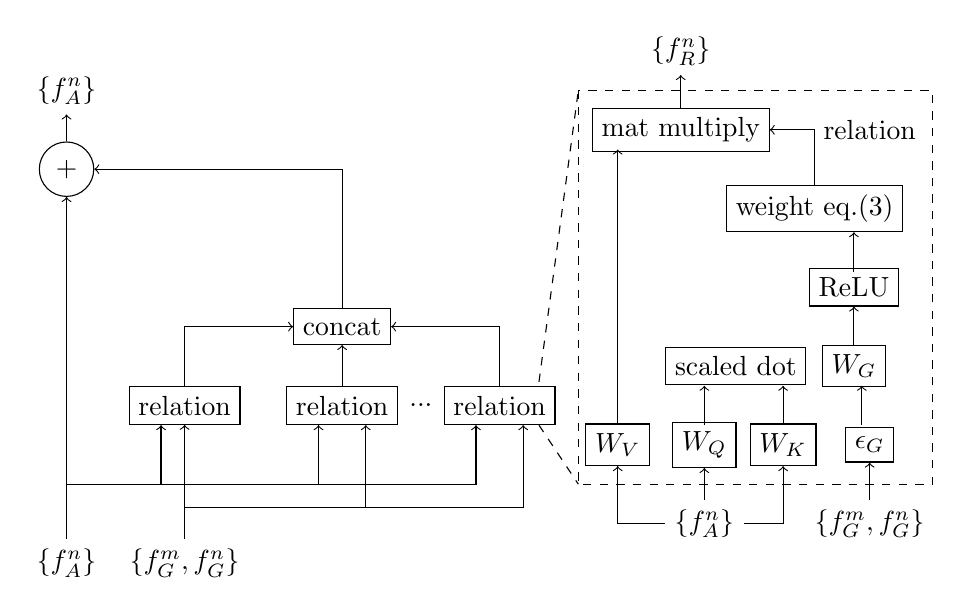
\begin{tikzpicture}
    \node [draw,rectangle](a)at(0,0){concat};
    \node [draw,rectangle](b)at(0,-1){relation};
    \node [draw,rectangle](c)at(-2,-1){relation};
    \node (d)at(1,-1){...};
    \node [draw,rectangle](e)at(2,-1){relation};
    \node [draw,circle](f)at(-3.5,2){+};
    \node (g)at(-3.5,3){$\{f_A^n\}$};
    \node (h)at(-3.5,-3){$\{f_A^n\}$};
    \node (i)at(-2,-3){$\{f_G^m,f_G^n\}$};
    \node [draw,rectangle](j)at(4.3,2.5){mat multiply};
    \node [draw,rectangle](k)at(6,1.5){weight eq.(3)};
    \node [draw,rectangle](l)at(6.5,0.5){ReLU};
    \node [draw,rectangle](m)at(5,-0.5){scaled dot};
    \node [draw,rectangle](n)at(3.5,-1.5){$W_V$};
    \node [draw,rectangle](o)at(4.6,-1.5){$W_Q$};
    \node [draw,rectangle](p)at(5.6,-1.5){$W_K$};
    \node [draw,rectangle](q)at(6.5,-0.5){$W_G$};
    \node [draw,rectangle](r)at(6.7,-1.5){$\epsilon_G$};
    \node (s)at(6.7,2.5){relation};
    \node (t)at(4.3,3.5){$\{f_R^n\}$};
    \node (u)at(4.6,-2.5){$\{f_A^n\}$};
    \node (v)at(6.7,-2.5){$\{f_G^m,f_G^n\}$};

    \draw [dashed](3,3) rectangle (7.5,-2);
    \draw [dashed](2.5,-0.7)--(3,3);
    \draw [dashed](2.5,-1.25)--(3,-2);

    \draw [->](node cs:name=a,angle=90)|-(f);
    \draw [->](node cs:name=b,angle=90)--(a);
    \draw [->](node cs:name=c,angle=90)|-(a);
    \draw [->](node cs:name=e,angle=90)|-(a);
    \draw [->](node cs:name=f)--(g);
    \draw [->](node cs:name=h)--(f);
    \draw	[->](node cs:name=i,angle=90)--(c);
    \draw [->](-3.5,-2) -|(-2.3,-1.25);
    \draw [->](-3.5,-2) -|(-0.3,-1.25);
    \draw [->](-3.5,-2) -|(1.7,-1.25);
    \draw [->](-2,-2.3) -|(0.3,-1.25);
    \draw [->](-2,-2.3) -|(2.3,-1.25);
    \draw [->](3.5,-1.25)--(3.5,2.25);
    \draw [->](4.6,-1.25)--(4.6,-0.75);
    \draw [->](5.6,-1.25)--(5.6,-0.75);
    \draw [->](6.6,-1.25)--(6.6,-0.75);
    \draw [->](q)--(l);
    \draw [->](6.5,0.7)--(6.5,1.2);
    \draw [->](k)|-(j);
    \draw [->](j)--(t);
    \draw [->](u)-|(n);
    \draw [->](u)--(o);
    \draw [->](u)-|(p);
    \draw [->](v)--(r);
\end{tikzpicture}

% Define block styles
\tikzstyle{decision} = [diamond, draw, fill=blue!20,
text width=4.5em, text badly centered, node distance=3cm, inner sep=0pt]
\tikzstyle{block} = [rectangle, draw, fill=blue!20,
text width=5em, text centered, rounded corners, minimum height=4em]
\tikzstyle{line} = [draw, -latex']
\tikzstyle{cloud} = [draw, ellipse,fill=red!20, node distance=3cm,
minimum height=2em]

\begin{tikzpicture}[node distance = 2cm, auto]
    % Place nodes
    \node [block] (init) {initialize model};
    \node [cloud, left of=init] (expert) {expert};
    \node [cloud, right of=init] (system) {system};
    \node [block, below of=init] (identify) {identify candidate models};
    \node [block, below of=identify] (evaluate) {evaluate candidate models};
    \node [block, left of=evaluate, node distance=3cm] (update) {update model};
    \node [decision, below of=evaluate] (decide) {is best candidate better?};
    \node [block, below of=decide, node distance=3cm] (stop) {stop};
    % Draw edges
    \path [line] (init) -- (identify);
    \path [line] (identify) -- (evaluate);
    \path [line] (evaluate) -- (decide);
    \path [line] (decide) -| node [near start] {yes} (update);
    \path [line] (update) |- (identify);
    \path [line] (decide) -- node {no}(stop);
    \path [line,dashed] (expert) -- (init);
    \path [line,dashed] (system) -- (init);
    \path [line,dashed] (system) |- (evaluate);
\end{tikzpicture}

\end{document}